\chapter{Appendices} \label{appA}

\section{Conference presentations for proposed investigations}
I have presented the work contained in this proposal at many conferences where I have gotten feedback and suggestions from others within the field. I list them here in relation to each project\\
\\
OCI Investigations:
\begin{itemize}
    \item April 2024; Copper Mountain Conference on Iterative Methods\\
    Presentation Title: Dynamic and Deterministic Neutron Transport on GPUs using One-cell Inversion
    \item August 2023; M\&C 2023\\
    Presentation Title: Exploring One-Cell Inversion Method for Transient Transport on GPU.
\end{itemize}
Hybrid-Delta Tracking Schemes
\begin{itemize}
    \item M\&C 2023\\
    Presentation Title: Hybrid-Delta Tracking on a Structured Mesh in MCATK.
\end{itemize}
Acceleration and Abstraction of Python
\begin{itemize}
    \item July 2024; Scientific Computing in Python 2024\\
    Presentation Title: Monte Carlo/Dynamic Code: Performant and Portable High-Performance Computing at Scale via Python and Numba 
    \item April 2024; Sustainable Scientific Software Conference\\
    Presentation Title: High Performance Python for Rapid Methods Development in Monte Carlo / Dynamic Code
    \item July 2022\\
    Presentation Title: Hardware Code Generation Techniques for Accelerating Python
    \item June 2022 Annual meeting of the ANS\\
    Presentation Title: Automatic Hardware Code Generation for Neutron Transport Applications
\end{itemize}

\section{Performant and Portable Monte Carlo Neutron Transport via Numba}
\label{app:cise}

This paper was submitted to \textit{IEEE Computing in Science and Engineering} on September 3rd 2024. 
I have not received a response.
A preprint was posted to arxiv and has been the assigned the DOI 10.48550/arXiv.2409.04668.

This work was done as part of my position in the Center for Exascale Monte Carlo Neutron Transport (CEMeNT).
%My coauthors are all members of the Center for Exascale Monte Carlo Neutron Transport (CEMeNT) includes
%\begin{itemize}
%    \item Ilham Variansyah, PhD (committee member)
%    \item Braxton Cuneo, PhD
%    \item Todd S. Palmer, PhD (committee member)
%    \item Kyle E. Niemeyer, PhD (advisor)
%\end{itemize}
%As MC/DC is the primary deliverable of CEMeNT it is a deeply combative effort.


%\subsection{My work}
%I was the primary author and as such drafted the whole paper.
%I received significant edits from all my co authors who all contributed to the work.
%I collected the data

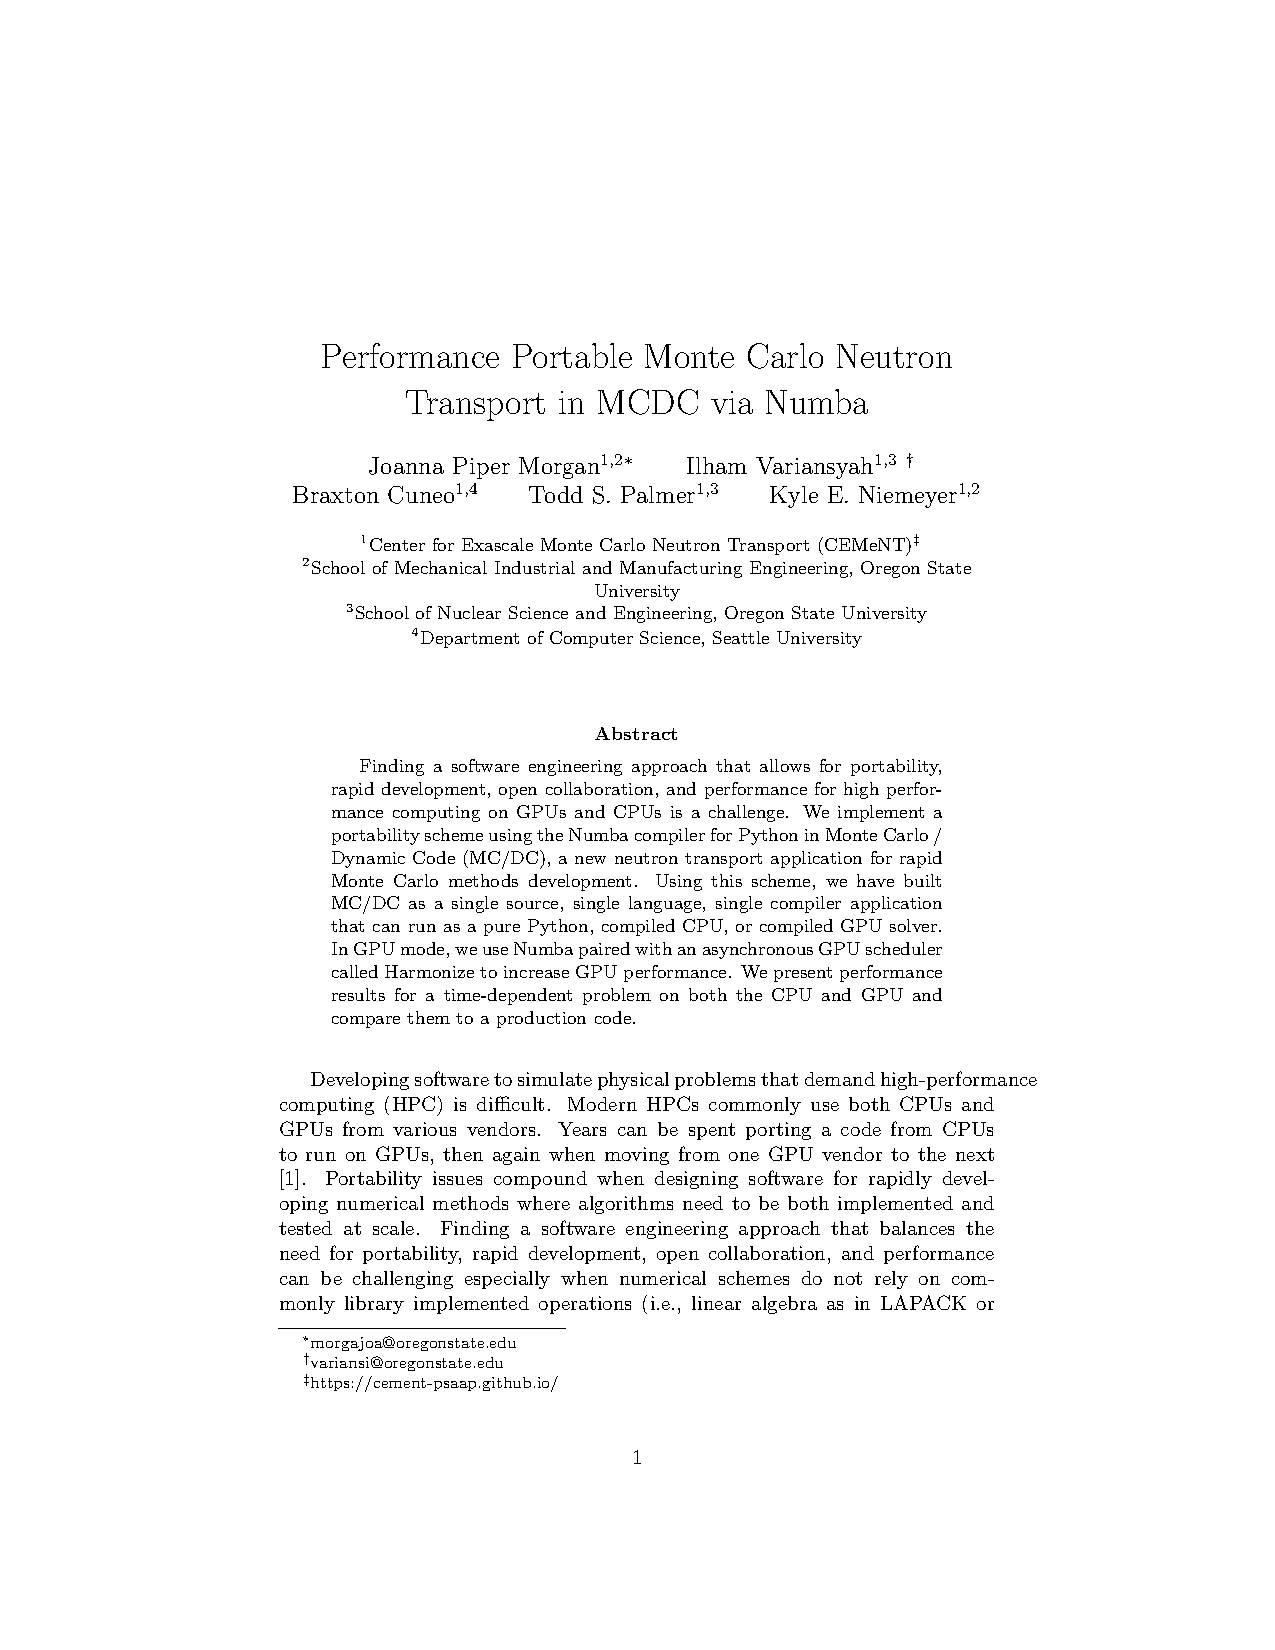
\includepdf[pages=-]{appendix/ana_numba_mcdc.pdf}


\section{Hybrid-Delta Tracking on a Structured Mesh in MCATK}

This work was reviewed and published in the \textit{Preceding of International Conference on Mathematics and Computational Methods Applied to Nuclear Science and Engineering} 2023 and was done as part of my work at Los Alamos National Laboratory.

%\begin{itemize}
%    \item Travis J. Trahan, PhD
%    \item Timothy P. Burke, PhD
%    \item Collin J. Josey, PhD
%    \item Kyle E. Niemeyer, PhD
%\end{itemize}

\label{app:hybridmcatk}
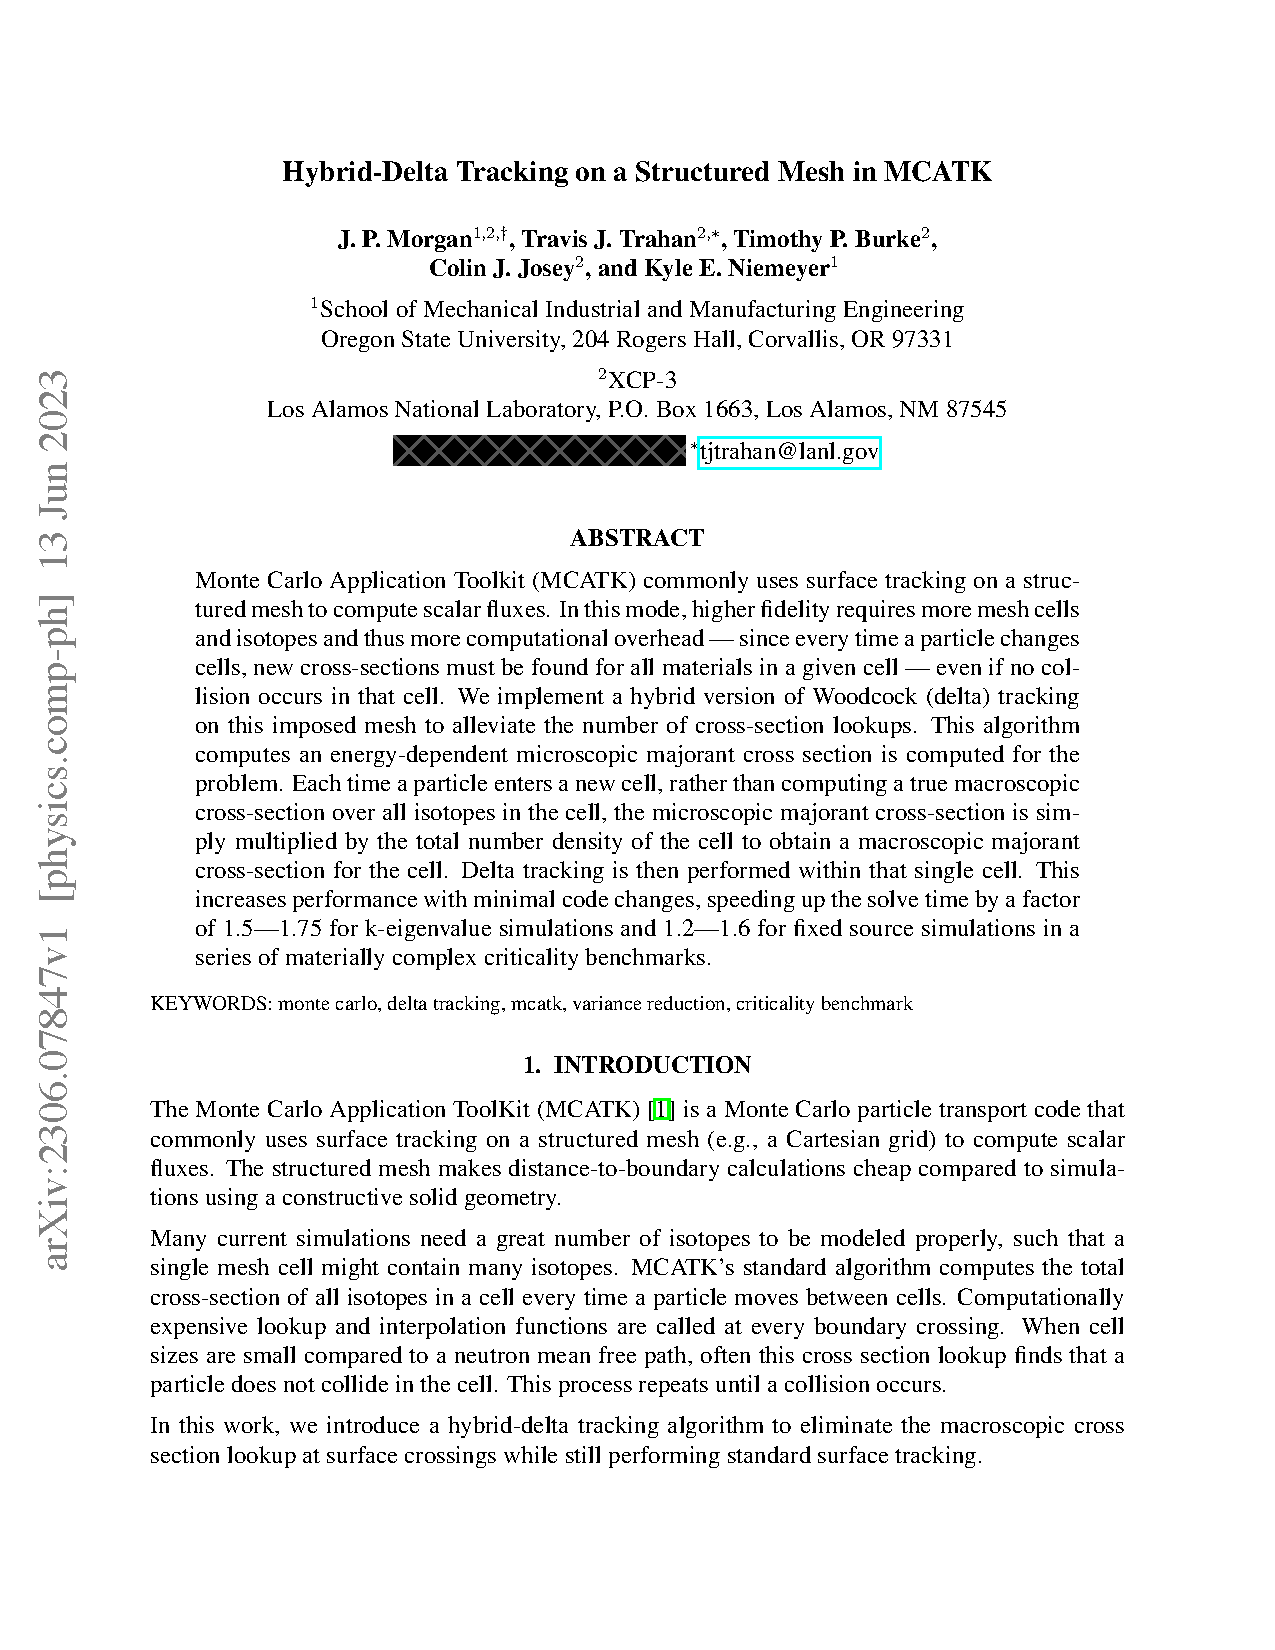
\includepdf[pages=-]{appendix/delta_tracking_mcatk.pdf}

\section{Draft: Therefore paper}
\label{app:therefore}

This is a rough draft of work to be submitted targeting the special edition of the \textit{Journal of Nuclear Science and Engineering} on Time Dependent Transport and Radiative Transfer.
Again my coauthors are all members of CEMeNT with a potential additional co-author who was my mentor at a previous internship at Advanced Micro Devices (AMD).

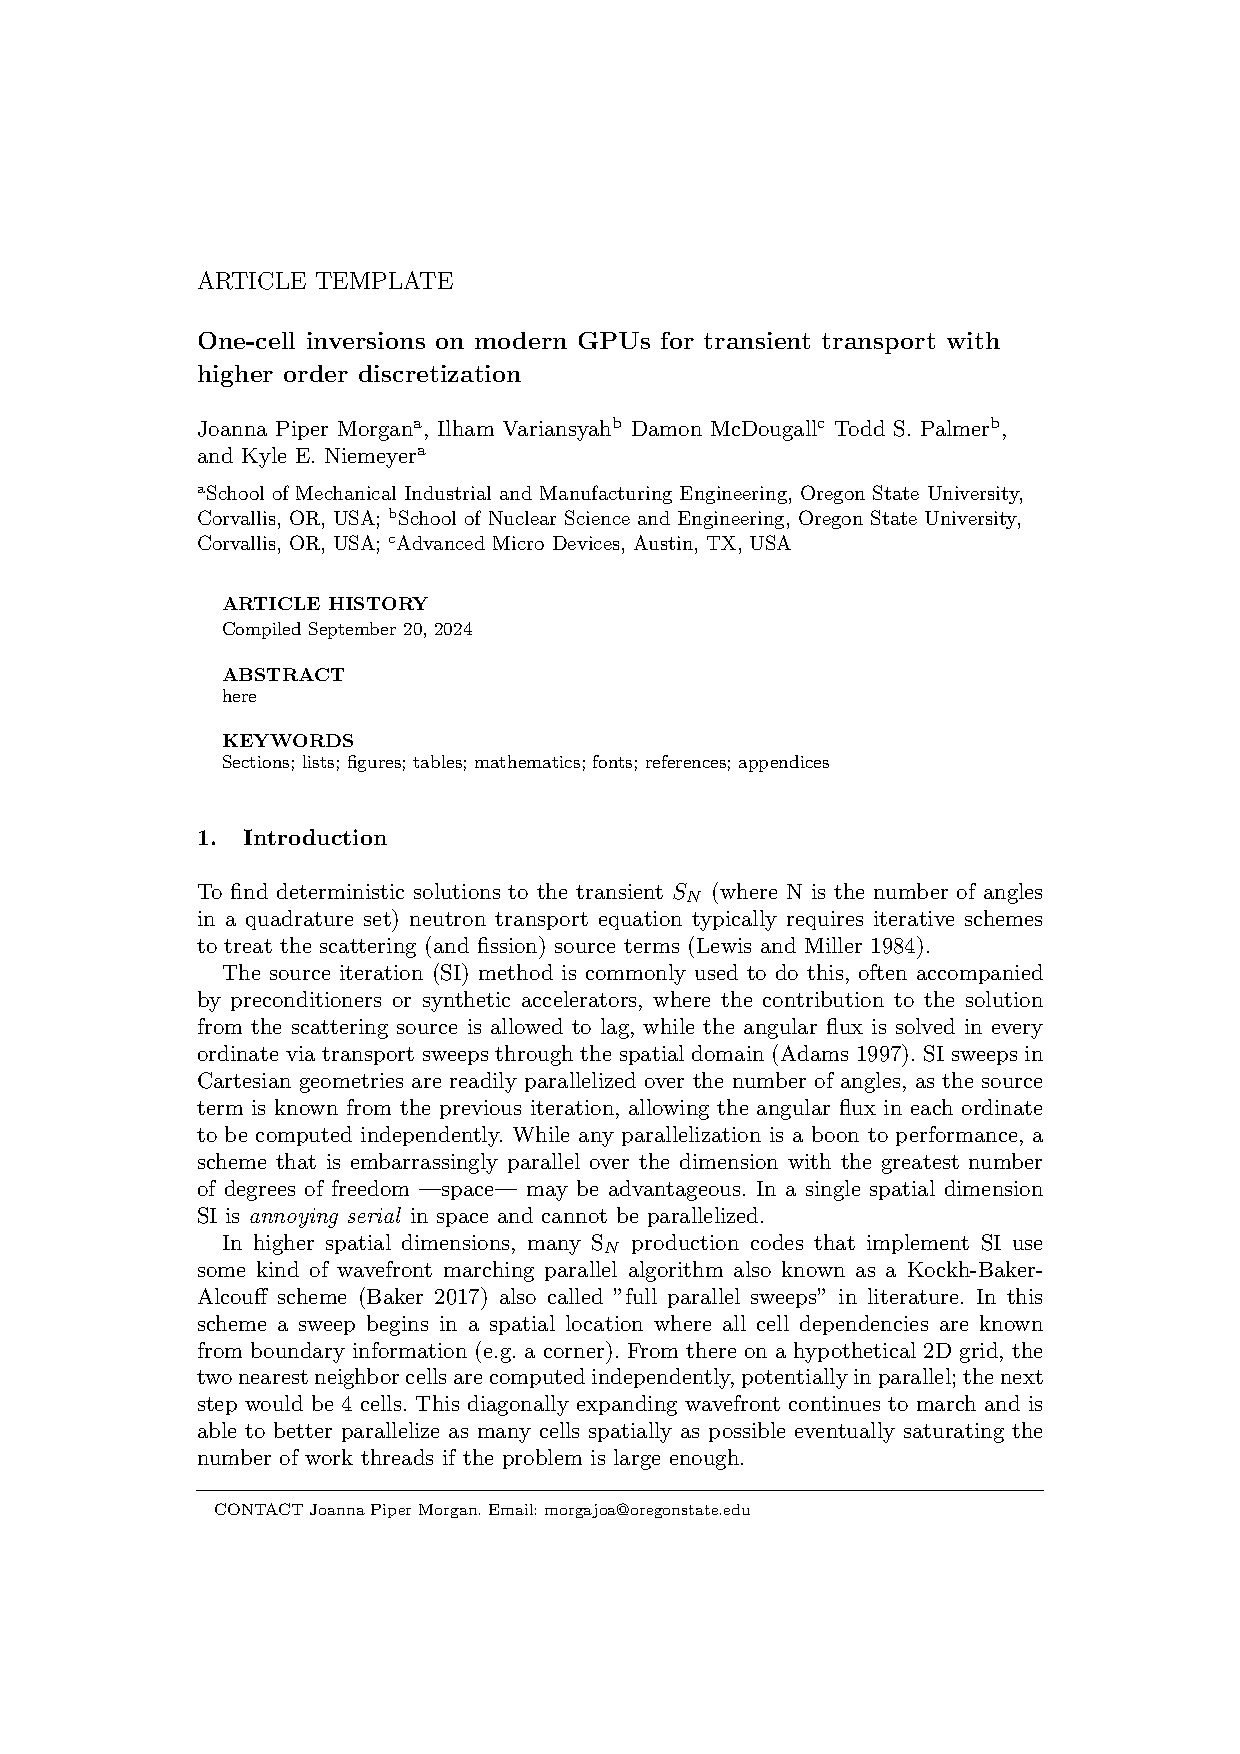
\includepdf[pages=-]{appendix/ThereforePaper.pdf}